\begin{figure}[htbp]
\centering
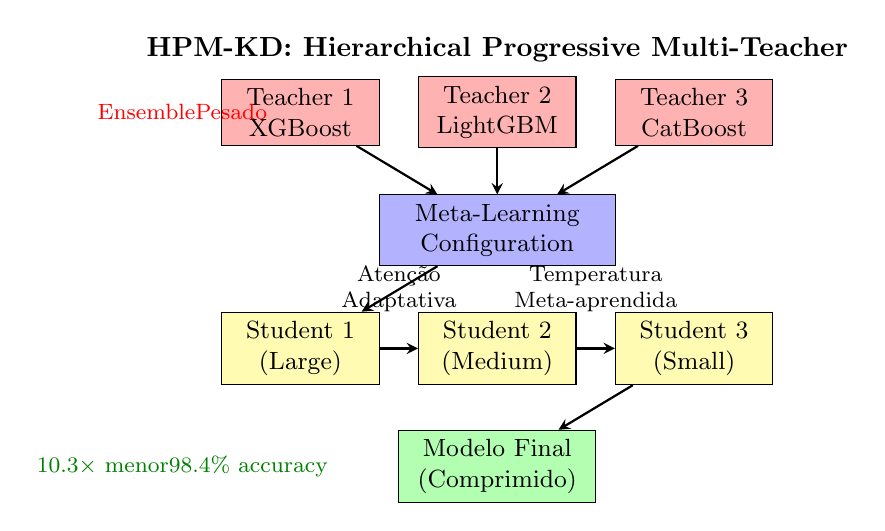
\begin{tikzpicture}[
    node distance=1.5cm,
    box/.style={rectangle, draw, minimum width=2cm, minimum height=0.8cm, align=center, font=\small},
    arrow/.style={->, >=stealth, thick},
    label/.style={font=\footnotesize}
]

% Teacher models
\node[box, fill=red!30] (t1) at (0,0) {Teacher 1\\XGBoost};
\node[box, fill=red!30] (t2) at (2.5,0) {Teacher 2\\LightGBM};
\node[box, fill=red!30] (t3) at (5,0) {Teacher 3\\CatBoost};

% Meta-learning config
\node[box, fill=blue!30, minimum width=3cm] (meta) at (2.5,-1.5) {Meta-Learning\\Configuration};

\draw[arrow] (t1) -- (meta);
\draw[arrow] (t2) -- (meta);
\draw[arrow] (t3) -- (meta);

% Progressive distillation
\node[box, fill=yellow!30] (s1) at (0,-3) {Student 1\\(Large)};
\node[box, fill=yellow!30] (s2) at (2.5,-3) {Student 2\\(Medium)};
\node[box, fill=yellow!30] (s3) at (5,-3) {Student 3\\(Small)};

\draw[arrow] (meta) -- (s1);
\draw[arrow] (s1) -- (s2);
\draw[arrow] (s2) -- (s3);

% Attention mechanism
\node[label, align=center] at (1.25,-2.25) {Atenção\\Adaptativa};
\node[label, align=center] at (3.75,-2.25) {Temperatura\\Meta-aprendida};

% Final model
\node[box, fill=green!30, minimum width=2.5cm] (final) at (2.5,-4.5) {Modelo Final\\(Comprimido)};

\draw[arrow] (s3) -- (final);

% Annotations
\node[label, text=red] at (-1.5,0) {Ensemble\\Pesado};
\node[label, text=green!50!black] at (-1.5,-4.5) {10.3$\times$ menor\\98.4\% accuracy};

% Title
\node[font=\bfseries] at (2.5,0.8) {HPM-KD: Hierarchical Progressive Multi-Teacher};

\end{tikzpicture}
\caption{Workflow do HPM-KD Framework. Múltiplos teachers (ensemble) são destilados progressivamente através de estudantes de tamanho decrescente, usando meta-learning para otimizar configurações (temperatura, peso de atenção). Resultado: compressão 10.3$\times$ com 98.4\% de retenção de acurácia.}
\label{fig:hpmkd_workflow}
\end{figure}
